\documentclass[11pt]{article}
 
\usepackage[margin=1in]{geometry} 
\usepackage{amsmath,amsthm,amssymb}
\usepackage{graphicx} 
\usepackage{blkarray}
\usepackage{amsmath}




\newcommand{\N}{\mathbb{N}}
\newcommand{\Z}{\mathbb{Z}}
 
\newenvironment{problem}[2][Problem]{\begin{trivlist}
\item[\hskip \labelsep {\bfseries #1}\hskip \labelsep {\bfseries #2.}]}{\end{trivlist}}
\newenvironment{lemma}[2][Lemma]{\begin{trivlist}
\item[\hskip \labelsep {\bfseries #1}\hskip \labelsep {\bfseries #2.}]}{\end{trivlist}}
\newenvironment{exercise}[2][Exercise]{\begin{trivlist}
\item[\hskip \labelsep {\bfseries #1}\hskip \labelsep {\bfseries #2.}]}{\end{trivlist}}

\newenvironment{question}[2][Question]{\begin{trivlist}
\item[\hskip \labelsep {\bfseries #1}\hskip \labelsep {\bfseries #2.}]}{\end{trivlist}}
\newenvironment{corollary}[2][Corollary]{\begin{trivlist}
\item[\hskip \labelsep {\bfseries #1}\hskip \labelsep {\bfseries #2.}]}{\end{trivlist}}

\usepackage{indentfirst}
\linespread{1.2}     % 调整间距
\setlength{\parindent}{0pt}

\begin{document}

 
% --------------------------------------------------------------
%                         Start here
% --------------------------------------------------------------
 
\title{Homework 4 DS-GA 1002 }%replace X with the appropriate number
\author{Yuhao Zhao\\ %replace with your name
N17578783} %if necessary, replace with your course title
 
\maketitle
\begin{problem}{1}
\end{problem}
(a) The Markov transition matrix for  this problem is  :
\[P = 
    \begin{blockarray}{ccc}
     &\text{Made the next} & \text{didn't make the next}\\
    \begin{block}{c(cc)}
    \text{Made the shot} & 0.6  &0.4 \\
    \text{Didn't make the shot}  & 0.3 &0.7 \\
    \end{block}
    \end{blockarray}
\]
The probability that he makes the 14th shot given he made 2nd and 12th is only relevant to the 13th shoot. The distribution of 13th shoot is only relevant to the 12th shoot. Let the distribution of ith shoot be $\pi_i$
$\pi_{13} = (0.6,0.4)$\\
$\pi_{14} = (0.6,0.4)  \left( \begin{array}{cc}
0.6 &0.4 \\
0.3& 0.7\\
\end{array} \right) = (0.48,0.52)$ \\
The probability that he makes the 14th shoot is 0.48\\

(b) We know that $\pi_{1} = (0.4,0.6)$. Let A be that  he made the first, B be that he didn't made the 3rd and C be that he didn't made 12th. We know that $P(A|B,C) = P(A|B)$ from the Markov property.\\
$P(A|B) \times P(B) = P(B|A) \times P(A), P(B|A) = 0.52,P(A) = 0.4$\\
$\pi_3= \pi_{1}  \left( \begin{array}{cc}
0.6 &0.4 \\
0.3& 0.7\\
\end{array} \right)^2 = (0.4,0.6)  \left( \begin{array}{cc}
0.6 &0.4 \\
0.3& 0.7\\
\end{array} \right)^2 = (0.426 ,0.574), P(B) = 0.574$\\
Therefore,the probability is $P(A|B) = \frac{0.52 \times 0.4}{0.574} \approx 0.3623693$\\

(c) Let K be the number of shots he made in a row. \\
$P(K = k| \text{made the first}) = 0.6^{k} *0.4, P(K = k| \text{didn't make the first}) = 0.3*0.6^{k-1} *0.4$ \\
$E(k) = \sum_{k = 1}^{\infty} k(0.4\times 0.6^{k} \times 0.4 + 0.6 \times 0.3\times 0.6^{k-1} \times 0.4)  = \sum_{k = 1}^{\infty} 0.16k\times 0.6^k + 0.072k\times 0.6^{k-1}$\\
$ = \sum_{k = 1}^{\infty} 0.28k \times 0.6^{k} = 0.28 \times \frac{0.6}{(1 - 0.6)^2} = 1.05$\\

\pagebreak

\begin{problem}{2}
\end{problem}
(a) $P_N(N = n) = \sum_{k =0}^{n} (\frac{1}{30} {n \choose k } (\frac{1}{4})^k (\frac{3}{4})^{n-k} +\frac{1}{60} {n \choose k } (\frac{4}{5})^k (\frac{1}{5})^{n-k} ) =  \frac{1}{30} + \frac{1}{60} = \frac{1}{20}$\\
 $P_C(C = \frac{1}{4}) = \sum_{n = 0}^{20}\sum_{k =0}^{n} \frac{1}{30} {n \choose k } (\frac{1}{4})^k (\frac{3}{4})^{n-k} = \frac{1}{30} \times 20 = \frac{2}{3}$,\\ Since C can only be $\frac{1}{4} or \frac{4}{5}, P_C(C = \frac{4}{5}) = 1 - \frac{2}{3} =\frac{1}{3} $\\
 N and C are independent,since P(N,C) = P(N)P(C), in particular:\\
% $P(N|C = \frac{1}{4}) =  \sum_{k =0}^{n} \frac{1}{30} {n \choose k } (\frac{1}{4})^k (\frac{3}{4})^{n-k} = \frac{1}{30} \neq P(N) = \frac{1}{20}$ 	\\
 $P(N,C = \frac{1}{4}) =  \sum_{k =0}^{n} \frac{1}{30} {n \choose k } (\frac{1}{4})^k (\frac{3}{4})^{n-k} = \frac{1}{30} = \frac{1}{20} \times \frac{2}{3} = P(n)P(C = \frac{1}{4})$\\
  $P(N,C = \frac{4}{5}) = \sum_{k =0}^{n} \frac{1}{60} {n \choose k } (\frac{4}{5})^k (\frac{1}{5})^{n-k} = \frac{1}{60} = \frac{1}{20} \times \frac{1}{3} = P(n)P(C = \frac{4}{5})$\\
 
 (b) C is the probability of a person taking taxi to work in a particular day, C = $\frac{1}{4}$ if he/she has a car, $\frac{4}{5}$ if she/he doesn't have a car. \\N is th number of days in a month the person has to work ($N < 20$).\\ K is the number of days that the person takes taxi to work.\\
 
(c) $P(N|K=k,C = \frac{1}{4})  =\frac{P(N,K,C=\frac{1}{4})}{P(K,C = \frac{1}{4})} = \frac{\frac{1}{30} {n \choose k } (\frac{1}{4})^k (\frac{3}{4})^{n-k}}{\sum_{n = k}^{20}\frac{1}{30} {n \choose k } (\frac{1}{4})^k (\frac{3}{4})^{n-k} }$\\
$P(N|K=k,C = \frac{4}{5})  =\frac{P(N,K,C=\frac{4}{5})}{P(K,C = \frac{4}{5})} = \frac{\frac{1}{60} {n \choose k } (\frac{4}{5})^k (\frac{1}{5})^{n-k}}{\sum_{n = k}^{20}\frac{1}{60} {n \choose k } (\frac{4}{5})^k (\frac{1}{5})^{n-k} }$\\
$P(N|K,C)$ is the probability of the number of days that the person need to work given he has car or not and number of days that he go to work by taxi.\\

(d)

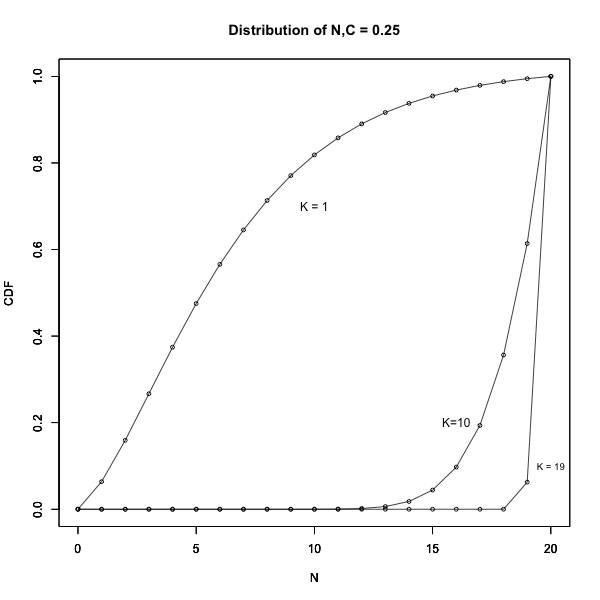
\includegraphics[height = 3.3in]{Q2_d_1} 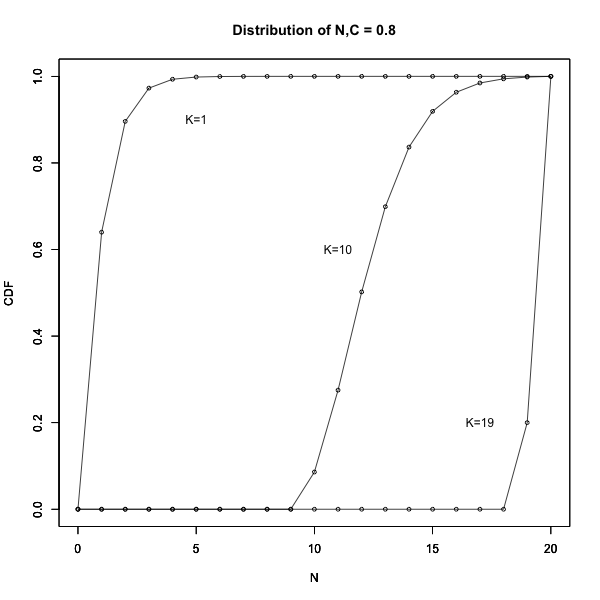
\includegraphics[height = 3.3in]{Q2_d_2}\\
For my example, on the one hand,for the same person, the more days that he/she takes taxi to work, the more days she need to work per month. Although this is common sense, but it proves the model is valid.\\
On the other hand, given the same number of days that two person taking taxi to work, the person who has a car has higher probability to work more days than the person who doesn't have a car.\\

\begin{problem}{3}
\end{problem}
(a) Let the number of packets arriving at the router be X, and the number of packets routed through connection 1 be Y. The model to this problem is that: $X \sim Poisson(\lambda), Y|X \sim Binomial(X,p)$\\
$E(Y) =E(E(Y|X))  = \sum_{x = 0}^{\infty} (px) \times p_X(x)  = p \sum_{x = 0}^{\infty} x \times p_X(x)  = p \times E_X(x) = \lambda p $ \\
$Var(Y) = E(Var(Y|X)) + Var(E(Y|X)) = \sum_{0}^{\infty} p(1-p)x \times p_X(x) + Var_x(px) = p(1- p)E(x) + p^2Var(x) = p(1- p) \lambda + p^2\lambda = \lambda p$\\

(b) $P(Y = y) = \sum_{K =y}^{\infty} P(Y =y|k)\times  p_X(k) = \sum_{y}^{\infty} { k \choose y}p^y(1-p)^{k-y} \times \frac{\lambda^k e^{-\lambda}}{k!}\\ = \sum_{y}^{\infty} \frac{1}{y!(k-y)!} \frac{(\lambda p)^y}{\lambda^y} (1 - p)^{k-y}\lambda^x e^{-\lambda  } = \frac{e^{-\lambda}}{y!}(\lambda p)^{y} \sum_{y}^{\infty} \frac{(\lambda (1-p))^{k-y}}{(k-y)!} =\frac{e^{-\lambda}}{y!}(\lambda p)^{y} \sum_{k = 0}^{\infty} \frac{(\lambda (1-p))^{k}}{k!}$\\
$\sum_{k = 0}^{\infty} \frac{(\lambda (1-p))^{k}}{k!}$ is the Taylor expansion of $e^{\lambda (1- p)}$\\
Therefore, $P(Y = y) = \frac{e^{-\lambda}}{y!}(\lambda p)^{y} e^{\lambda (1- p)} = e^{-\lambda p} \frac{(\lambda p)^y}{y!} \sim poisson(\lambda p)  $

\begin{problem}{4}
\end{problem}
 (a) We want to find $\Delta$ such that, $P(|X_i -d_i| > \Delta) < 1 \% $.\\
 We know that by chebyshev inequality, $P(|Z_i - 0| \geq 10 \sigma ) \leq  \frac{1}{10^2} = 0.01$, $\Delta  = 10\sigma = 10$ 
 \\

 (b) $|Y_i - d_i| = |\frac{1}{m} \sum_{i-m+1}^{i} Xj - di |= |\frac{1}{m}  \sum_{i-m+1}^{i} Xj + \frac{1}{m}(d_i - d_{i-1}) + \frac{1}{m} (d_i - d_{i-2}) + ... + \frac{1}{m} (d_i - d{i-m+1})|$\\
 Since the max speed is 2 m/s, $d_i - d_j \leq 2(i-j)$\\
 Therefore,by triangular inequality ,\\
  RHS $\leq  | \frac{1}{m}\sum_{i-m+1}^{i} Xj| + | \frac{1}{m} \sum_{i-m+1}^{i-1} d_i - d_{j} |  \leq  |\frac{1}{m}\sum_{i-m+1}^{i} Xj| + |\frac{2}{m}(1 + 2 +... +m-1)|$\\
  RHS $\leq |\frac{1}{m}\sum_{i-m+1}^{i} Xj| + \frac{m(m-1)}{m}$\\
  Since $X_j$ are iid normal(0,1), $\frac{1}{m}\sum_{i-m+1}^{i} Xj ~\sim N(0, \frac{1}{\sqrt{m}})$\\
  By Chebshev inequality: $P(|\frac{1}{m}\sum_{i-m+1}^{i} Xj - 0| \geq 10 \frac{1}{\sqrt{m}} )\leq 0.01\\ \to P(|\frac{1}{m}\sum_{i-m+1}^{i} Xj - 0| + (m-1) \geq 10 \frac{1}{\sqrt{m}} +(m-1)) \leq 0.01$ \\
  Since $0 < |Y_i - d_i |\leq|\frac{1}{m}\sum_{i-m+1}^{i} Xj - 0| + (m-1), P(|Y_i - d_i| \geq \Delta_2) \leq P(|\frac{1}{m}\sum_{i-m+1}^{i} Xj - 0| + (m-1) \geq \Delta_2) $\\ 
  Therefore, let $\Delta_2 = 10 \frac{1}{\sqrt{m}} +(m-1)$, $P(|Y_i - d_i| > \Delta_2 ) < 0.01$\\
  \\
 
  (c) Let m = 4, $\Delta_2 = 10\times 0.5+3 = 8$. She use m = 4 because $\sqrt{4}$ is an integer.\\ 
  \\
  
  (d) We want to minimize $\Delta_2$. $\Delta_2(m) = \frac{10}{\sqrt{m}} + m-1\\
  \frac{d \Delta}{dm} = 1- \frac{5}{m^{3/2}} = 0, m = 5^{2/3} \approx 2.92$.\\
  Since m can only be integer, $\Delta_2(2) \approx 8.07, \Delta_2(3) \approx 7.77$. The best precision at be attained at m = 3, which is $\frac{10}{\sqrt{3}} + 2$\\

  
 \pagebreak
  
  \begin{problem}{5}
  \end{problem}
  (a)We can define $E(X_I| X_J)$ as  $E(X_I| X_J) = \int_{X_I} X_I f_{X_I|X_J}(X_I|X_J)d X_I$. It'a a random vector.\\
  $E(E(X_I| X_J)) = \int_{X_J} E(X_I| X_J) f(X_J)dX_J =  \int_{X_J} \int_{X_I} X_I f_{X_I|X_J}(X_I|X_J)d X_If(X_J)dX_J$\\
  Since $f_{X_I|X_J} = \frac{f_{X_I,X_J}}{f_{X_J}}$\\
  Therefore, $E(E(X_I| X_J)) = \int_{X_J} E(X_I| X_J) f(X_J)dX_J =  \int_{X_J} \int_{X_I} X_I \frac{f_{X_I,X_J}}{f_{X_J}} f(X_J) d X_IdX_J$\\
   = $\int_{X_J} \int_{X_I} X_I f_{X_I,X_J} d X_IdX_J =  \int_{X_I}X_I \int_{X_J}  f_{X_I,X_J} d X_JdX_I = \int_{X_I} X_I f_{X_I} dX_I  =E(X_I)$\\
   
   (b) $E(K) = E(E(K|N,C))$\\
   $K|N,C $ is just a binomial distribution with N = n and p = c.\\
   $E(K|N,C) = \frac{n}{4}, c = \frac{1}{4}, and = \frac{4n}{5}, c = \frac{4}{5}$   \\
   $P_{N,C}(n, \frac{1}{4}) = \frac{1}{30},P_{N,C}(n, \frac{4}{5}) = \frac{1}{60} $\\
   Therefore, $E(K) = \sum_{0}^{20} \frac{n}{4} \times \frac{1}{30} + \frac{4n}{5} \times \frac{1}{60} = 4.55$\\
   
   $E(K^2|N,C) = Var(K|N,C) + E(E(K|N,C))^2$\\
   for $c = \frac{1}{4}$, $E(K^2|N,C)  = \frac{n}{4}(\frac{3}{4} + \frac{n}{4})$\\
   for $c = \frac{4}{5}, E(K^2|N,C) = \frac{4n}{5}(\frac{1}{5}+ \frac{4n}{5})$\\
   Therefore, $E(K^2) = E(E(K^2|C,N)) = \sum_{0}^{20} \frac{n}{4}(\frac{3}{4} + \frac{n}{4})\times \frac{1}{30} + \frac{4n}{5}(\frac{1}{5}+ \frac{4n}{5})\times \frac{1}{60} = 38.465 $\\
   $Var(K) = E(K^2) - E(K)^2 = 17.7625$
 


  





\end{document}